% !TeX encoding = UTF-8
% !TeX root = ../main.tex

\section{研究课题概述}

\begin{frame}{背景:编译器的中间语言}
  \textcolor{DarkBlue}{延续传递风格(Continuation-Passing Style, CPS)}
  \begin{itemize}
    \item CPS是\textcolor{Maroon}{函数式}编译器中常用的中间语言(Intermediate Representation, IR)。
    \item 每一步计算和控制流跳转都要被\textcolor{Maroon}{显式命名}。
    \item CPS中间语言有利于进行\textcolor{Maroon}{控制流分析}。
  \end{itemize}
  \vspace{2ex}
  \textcolor{DarkBlue}{静态单赋值(Static Single Assignment, SSA)}
  \begin{itemize}
    \item SSA是\textcolor{Maroon}{LLVM、GCC}等主流编译器基础设施常用的中间语言。
    \item 每一个变量都只能被\textcolor{Maroon}{赋值一次}。
    \item SSA中间语言有利于进行\textcolor{Maroon}{数据流分析}。
  \end{itemize}
\end{frame}

\begin{frame}{研究动机}
    \begin{itemize}
      \item SSA程序可以用函数式程序表示。CPS和SSA程序在结构上有对应之处。
      \item 目前\textcolor{Maroon}{没有}从CPS到SSA\textcolor{Maroon}{经过形式化验证}的转换。
      \item 我们希望经验证的函数式编译器能够利用SSA的优势。
    \end{itemize} 
    \begin{figure}
      \centering
      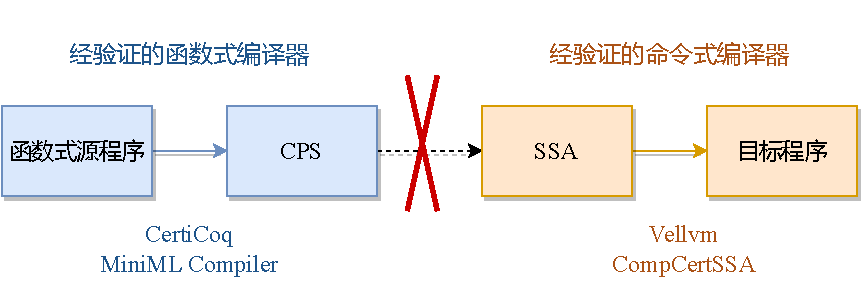
\includegraphics[width=0.8\linewidth]{figures/motiva.pdf}
      \label{fig:moti1}
    \end{figure}
\end{frame}

\begin{frame}{编译器验证技术}
  \textcolor{DarkBlue}{编译器形式化验证}常用技术:
  \begin{itemize}
    \item 基于逻辑关系的验证。与现有的经验证SSA基础设施所用方法不匹配。
    \item 基于\textcolor{Maroon}{模拟(simulation)}的验证。
  \end{itemize}
  \vspace{2ex}
  函数式语言与命令式语言的\textcolor{DarkBlue}{程序状态}组成部分\textcolor{DarkBlue}{差异较大}:
  \begin{itemize}
    \item \textcolor{Maroon}{CPS}:代码项,延续变量信息
    \item \textcolor{Maroon}{SSA}:程序计数器,符号表,调用栈...
  \end{itemize}
  想要使用模拟技术,需要把两种不同的程序状态正确地\textcolor{DarkBlue}{匹配}起来。
\end{frame}

\begin{frame}{主要贡献 1}
  \large
  设计并验证了\textcolor{DarkBlue}{CPS到SSA}语言的转换算法。
  \begin{figure}
    \centering
    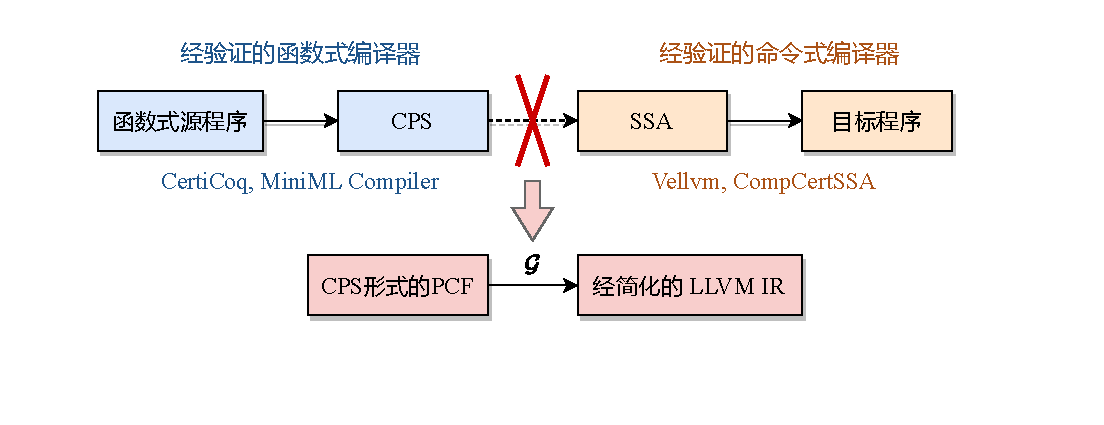
\includegraphics[width=0.95\linewidth]{figures/part.pdf}
  \end{figure}  
\end{frame}

\begin{frame}{主要贡献 2}
  \large
  利用该经验证的编译过程构建了\textcolor{DarkBlue}{PCF到LLVM IR}的函数式编译器。
  \begin{figure}
    \centering
    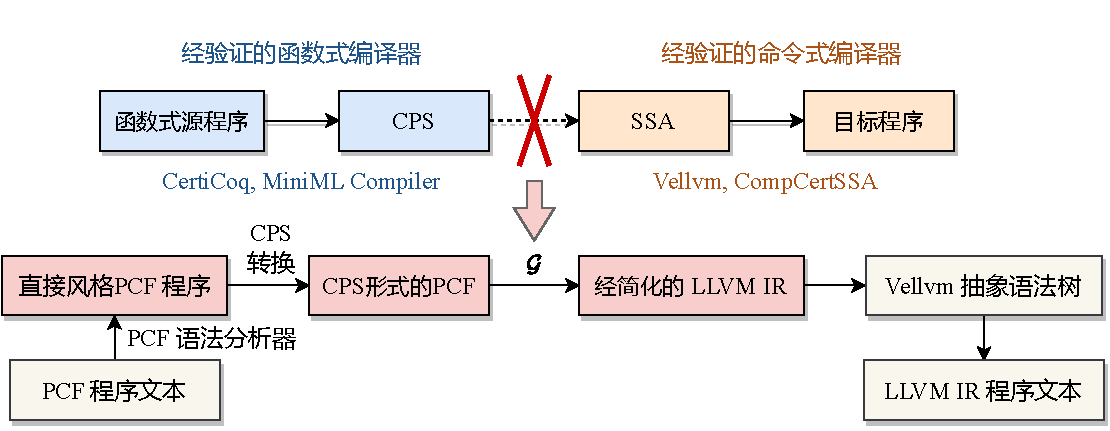
\includegraphics[width=0.95\linewidth]{figures/whole.pdf}
  \end{figure}  
\end{frame}


